\chapter{Исследовательская часть}

\section{Технические характеристики}

Технические характеристики устройства, на котором выполнялось тестирование:

\begin{itemize}
	\item операционная система: Windows 10;
	\item оперативная память: 16 Гб;
	\item процессор: Intel® Core™ i5-8259U;
	\item количество ядер: 4;
	\item количество логических процессоров: 8.
\end{itemize}

Во время тестирования ноутбук был включен в сеть питания и нагружен только встроенными приложениями окружения и системой тестирования.

\section{Пример работы программы}
На рисунке \ref{fig:work_example} приведен пример работы программы.
\clearpage
\begin{figure}[h!]
	
	\centering{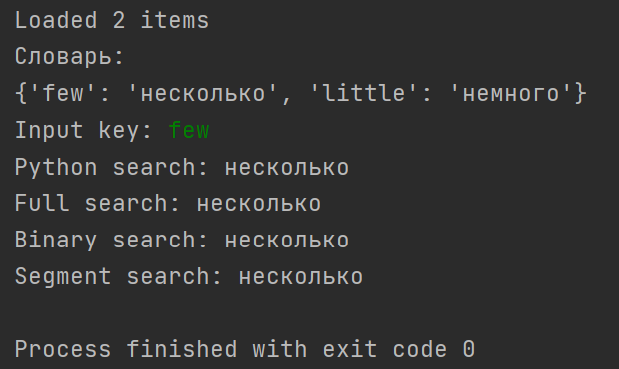
\includegraphics[scale=1]{inc/img/work_example.png}}
	
	\caption{Пример работы программы}
	
	\label{fig:work_example}
	
\end{figure}


\section{Количество сравнений}

На рисунках \ref{img:full_k}-\ref{img:segment_kg} приведены гистограммы с количеством сравнений (ось y), которые потребовались рассматриваемым реализациям алгоритмов поиска по ключам в словаре для того, чтобы найти нужный ключ (ось x). Все замеры производились в случае словаря, состоящего из 31 элемента. Для каждой реализации приведены две гистограммы, построенные по одним и тем же данным, но в первой ключи на оси x расположены в том порядке, в котором они хранились в словаре, а во второй -- упорядочены по убыванию потребовавшегося количества сравнений.

\clearpage
\img{120mm}{full_k}{Количество сравнений: полный перебор, сортировка по расположению}
\img{120mm}{full_kg}{Количество сравнений: полный перебор, сортировка по сравнениям}

\clearpage
\img{120mm}{binary_k}{Количество сравнений: бинарный поиск, сортировка по расположению}
\img{120mm}{binary_kg}{Количество сравнений: бинарный поиск, сортировка по сравнениям}

\clearpage
\img{120mm}{segment_k}{Количество сравнений: поиск в сегментированном словаре, сортировка по расположению}
\img{120mm}{segment_kg}{Количество сравнений: поиск в сегментированном словаре, сортировка по сравнениям}

\clearpage
Из рисунков \ref{img:full_k} и \ref{img:full_kg} видно, что количество сравнений, необходимых для поиска данного ключа полным перебором определяется только позицией ключа в словаре и равно этой позиции. Наименьшее количество сравнений (1) потребуется для самого первого ключа, наибольшее (N-количество элементов в словаре) - для последнего. Для определения того, что ключа нет в словаре, потребуется столько же сравнений, сколько и для худшего случая.

Из рисунков \ref{img:binary_k} и \ref{img:binary_kg} видно, что количество сравнений, необходимых для поиска данного ключа бинарным поиском также определяется позицией ключа в словаре, но здесь зависимость более сложная, так как надо учитывать еще и ход разбиения исходного словаря. Наименьшее количество сравнений (1) потребуется для серединного ключа, далее 2 сравнения для элементов на границе 1/4 и 3/4, а наибольшее - $(2*\log{(N+1)}) - 1$ (в данном примере для нечетных). Для определения того, что ключа нет в словаре, потребуется столько же сравнений, сколько и для худшего случая.

Из рисунков \ref{img:segment_k} и \ref{img:segment_kg} видно, что количество сравнений, необходимых для поиска данного ключа в сегментированном словаре определяется не только позицией ключа в своем сегменте, но и размером этого сегмента (так как наибольшие сегменты размещены ближе к началу). Наименьшее количество сравнений (2) потребуется для поиска самого первого ключа в самом большом сегменте, а наибольшее в общем случае определить нельзя: таковым может оказаться, например, ключ на <<неудачной>> позиции в самом большом сегменте или единственный ключ из самого маленького сегмента. 

Для определения того, что заданный ключ отсутсвтует в словаре, в случае поиска в сегментирванном словаре возможны два варианта. Если в словаре нет ключей, которые начинаются на ту же букву, что и искомый ключ, то понадобится столько сравнений, сколько сегментов в словаре. Если же такие ключи есть, то к количеству сравний, которое потребовалось для поиска нужного сегмента, нужно добавить количество сравнений, которое потребуется бинарному поиску для определения отсутсвия ключа в пределах сегмента.

Также для полноты картины на рисунках \ref{img:full2_k}-\ref{img:segment2_kg} приведены гистограммы, построенные для тех же алгоритмов по тому же принципу, но при словаре из 10000 элементов. 

\clearpage
\img{190mm}{full2_k}{Количество сравнений: полный перебор, сортировка по расположению, словарь из 10000 элементов}
\img{190mm}{full2_kg}{Количество сравнений: полный перебор, сортировка по сравнениям, словарь из 10000 элементов}

\clearpage
\img{190mm}{binary2_k}{Количество сравнений: бинарный поиск, сортировка по расположению, словарь из 10000 элементов}
\img{190mm}{binary2_kg}{Количество сравнений: бинарный поиск, сортировка по сравнениям, словарь из 10000 элементов}

\clearpage
\img{190mm}{segment2_k}{Количество сравнений: поиск в сегментированном словаре, сортировка по расположению, словарь из 10000 элементов}
\img{190mm}{segment2_kg}{Количество сравнений: поиск в сегментированном словаре, сортировка по сравнениям, словарь из 10000 элементов}

\clearpage
В таблице ~\ref{tab:cmp} приведены значения минимального (min), среднего (mean), медианного (median) и максимального (max) количества сравнений, которые потребовались рассатриваемым реализациям при поиске всех ключей в словаре из 10000 элементов. В таблице введены следующие обозначения алгоритмов: full - поиск полным перебором, binary - бинарный поиск, segment - поиск в сегментированном словаре.

\begin{table}[h!]
	\begin{center}
		\begin{tabular}{|c | c | c | c |}
			\hline
			 & full & binary & segment \\
			\hline
			min & 1 & 1 & 2 \\
			mean & 5000.5 & 23.7262 & 21.6744 \\
			median & 5000 & 25 & 22 \\
			max & 10000 & 27 & 29 \\
			\hline
		\end{tabular}
	\end{center}
	\caption{\label{tab:cmp} Количество сравнений.}
\end{table}



Таким образом, в общем случае наибольшее количество сравнений требуется в алгоритме полного перебора. Соотношение среднего, медианного и максимального количества сравнений в бинарном поиске и поиске в сегментированном словаре определяется размером словаря и количеством и размерами сегментов в сегментированном словаре.

\clearpage
\section{Сравнение трудоемкостей}

Рассмотрим трудоемкости реализаций при словаре с N ключами. Трудоемкость дается по количеству сравнений, которое потребовалось алгоритму для решения задачи.
%??? тут надо сказать про колво сравнений, по которым дана оценка

\begin{itemize}
	\item Поиск полным перебором
	\begin{itemize}
		\item Трудоемкость в среднем может быть рассчитана как математическое ожидание по формуле (\ref{for:brute}), где $\Omega$ -- множество всех возможных случаев.
		
		\begin{equation}
			\label{for:brute}
			\begin{aligned}
				\sum\limits_{i \in \Omega} p_i \cdot f_i = \frac{1}{N + 1} \cdot ((\sum\limits_{i \in [1, N]}i) + N) = \\
				= \frac{1}{N + 1} \cdot (\frac{1 + N}{2} \cdot N + N) \sim \frac{N}{2}
			\end{aligned}
		\end{equation}
			
		%\begin{equation}
		%\label{for:brute}
		%\begin{aligned}
			%\sum\limits_{i \in \Omega} p_i \cdot f_i = & (k_0 + k_1) \cdot \frac{1}{N + 1} + (k_0 + 2 \cdot k_1) \cdot \frac{1}{N+1} +\\
		%	& + (k_0 + 3 \cdot k_1) \cdot \frac{1}{N + 1} + (k_0 + Nk_1)\frac{1}{N + 1} + (k_0 + N \cdot k_1) \cdot \frac{1}{N + 1} =\\
		%& = k_0\frac{N+1}{N+1}+k_1+\frac{1 + 2 + \cdots + N + N}{N + 1} = \\
			%& = k_0 + k_1 \cdot \left(\frac{N}{N + 1} + \frac{N}{2}\right) = k_0 + k_1 \cdot \left(1 + \frac{N}{2} - \frac{1}{N + 1}\right)
		%\end{aligned}
	%\end{equation}
		
		\item Лучший случай - когда ключ стоит на первой позиции в словаре или отсутствует в нем. Тогда придется сравнить искомый ключ только один раз, а трудоемскость составит O(1).
		
		\item Худший случай - когда ключ стоит на последней позиции в словаре, и тогда придется сравнить искомый ключ с каждым ключом словаря, а трудоемкость составит O(n).
		
		\item Добавлять новый элемент в словарь можно на любую позицию, трудоемкость добваления O(1).

	\end{itemize}


	\item Бинарный поиск
	\begin{itemize}
	\item Трудоемкость в среднем составляет $O(\log{N})$~\cite{second_article}.
	
	\item Лучший случай - когда ключ стоит на серединной позиции в словаре, и тогда придется сравнить искомый ключ только один раз, а трудоемскость составит O(1).
	
	\item Первый худший случай - когда ключ стоит на такой позиции, что исходный словарь придется разбивать на части вплоть до того момента, когда левая и правая границы поиска совпадут. Тогда придется сравнить искомый ключ с каждым ключом словаря $2*\log{(N+1)} - 1$ раз и трудоемскость составит $O(\log{N})$. Вторым худшим случаем с той же трудоемкостью является ситуация, когда ключ отсутсвует в словаре.
	
	\item Добавлять новый элемент в словарь нужно так, чтобы он остался отсортированным, трудоемкость добваления в худшем случае O(N).
	\end{itemize}


	\item Поиск в сегментированном словаре
	\begin{itemize}
		\item Трудоемкость в среднем при множестве всех возможных случаев $\Omega$ может быть рассчитана по формуле (\ref{for:anal}). 
		\begin{equation}
			\label{for:anal}
			\sum_{i \in \Omega}{\left(f_{\text{выбор сегмента i-ого эл.}} + f_{\text{бинарный поиск i-ого эл.}}\right)} \cdot p_i \\ \sim i + \log{n_i},
		\end{equation} 
	%$O(\log{N})$~\cite{second_article}.
		где $n_i$ - количество элементов в i-ом сегменте
		\item Лучший случай - когда ключ стоит на первой позиции в самом большом сегменте словаря, и тогда придется сравнить искомый ключ только 2 раза, а трудоемскость составит O(1).
		
		\item Худший случай сильно зависит от того, как распределятся ключи по сегментам словаря -- насколько далеко от начала окажется нужный сегмент и насколько <<неудачной>> для бинарного поиска окажется позиция ключа в этом сегменте. Таковым может оказаться, например, ключ на <<неудачной>> позиции в самом большом сегменте или единственный ключ из самого маленького сегмента. 
	
		\item Для определения того, что заданный ключ отсутсвтует в словаре, в случае поиска в сегментирванном словаре возможны два варианта. Если в словаре нет ключей, которые начинаются на ту же букву, что и искомый ключ, то понадобится столько сравнений, сколько сегментов в словаре и трудоемкость составит N. Если же такие ключи есть, то к количеству сравний, которое потребовалось для поиска нужного сегмента, нужно добавить количество сравнений, которое потребуется бинарному поиску для определения отсутсвия ключа в пределах сегмента и трудоемкость составит $i + \log{n_i}$, где i-номер сегмента, начинающегося на ту же букву, $n_i$ - количество элементов в этом сегменте.
		
		\item Добавлять новый элемент в словарь нужно так, чтобы его сегменты остались отсортированы по размеру, а сегмент, в который попадет добавляемый ключ -- по лексикографическому порядку.
	\end{itemize}

\end{itemize}

%Трудоемкость определения того, что заданный ключ отсутсвтует в словаре в каждом алгоритме равна трудоемкости худшего случая.

\section{Сравнение времени выполнения реализаций алгоритмов}

Сравнивалось процессорное время работы реализаций алгоритмов поиска в словаре по ключу: алгоритма полного перебора, алогоитма бинарного поиска и алгоритма поиска в сегментированном словаре. Эти реализации сравнивались по времени работы при количестве ключей в словаре 100, 1000, 5000, 10000 и 40000.

Для каждого алгоритма и каждого количества ключей проводилось 2 замера времени. Первый был связан с поиском ключей, которые были в словаре, причем осуществлялся поиск каждого ключа, что позволило сымитировать равновозможность выбора ключа (время поиска всех ключей суммировалось). Второй замер был связан с поиском ключей, которых не было в словаре. Таких <<несуществующих>> ключей генерировалось столько, сколько всего ключей было в словаре (время поиска всех ключей также суммировалось).
 
Так как некоторые задачи выполняются достаточно быстро, а замеры времени имеют некоторую погрешность, они для каждой реализации, каждого объема словаря и каждого набора ключей для поиска выполнялись 10 раз, а затем вычислялось среднее время работы.
 

На рисунке \ref{img:time_all2} приведены результаты сравнения времени выполнения реализаций алгоритмов. На графике введены следующие обозначения: full\_x - алгоритм полного перебора, binary\_x - алгоритм бинарного поиска, segment\_x - алгоритм поиска в сегментированном словаре, x=e (exists) - время работы соответсвующего алгоритма при поиске существующих ключей, x=n (not exist) -- при поиске несуществующих ключей.

\clearpage
\img{120mm}{time_all2}{Сравнение времени работы реализаций в зависимости от объема словаря}

Как видно из графиков, и для поиска существующего ключа, и для определения того, что ключа в словаре нет, наибольшее количество процессорного времени требуется алгоритму полного перебора, наименьшее - поиску в сегментированном словаре. При рассмторении каждого алгоритма отдельно можно отметить, что для поиска существующих ключей требуется меньше времени, чем для определения того, что ключа в словаре нет.

Однако необходимо учитывать, что в случае бинарного поиска может понадобиться время на предварительную сортировку словаря, а в случае поиска в сегментированном словаре - на саму сегментацию словаря и сортировку значений внутри сегментов.

С увеличением размеров словаря разница во времени работы алгоритмов увеличивается.


%Также можно отметить тот факт, что при использовании алгоритма бинарного поиска и поиска в сегментированном словаре, время поиска существующего ключа меньше времени определения отсутсвия заданного ключа 




\clearpage
\section{Вывод из исследовательской части}

Таким образом, алгоритм полного перебора, как метод <<грубой силы>> в среднем требует больше процессорного времени для поиска ключа в словаре, но зато он не требует особого способа хранения словаря и дополнительной памяти, а новые элемента можно добавлять на любую позицию. Такой метод подходит для словаря небольших размеров.

С увеличением количества элементов в словаре стоит обращаться к менее простым методам поиска -- алгоритму бинарного поиска или к сегментации словаря с сортировкой сегментов по частотности обращенияя и последующим бинарным поиском в пределах сегмента. Но они потребуют дополнительных затрат: первый дополнительно потребует  хранения словаря в отсортированном виде, а второй -- отсортированности среди сегментов (подсегментов) и в пределах самих сегментов (подсегментов), а также дополнительной памяти.

Также при использовании сегментированного словаря необходимо провести анализ для определения наиболее подходящей структуры, количества сегментов и подсегментов, признаков для их сортировки.